\chapter{Calculating the Schemas}

Graph query engines often use single-machine (even single-threaded), search-based algorithms. Using these algorithms includes many tradeoffs:

\begin{itemize}
	\item They do not scale well for large graphs.
	\item They cannot run in parallel.
	\item They cannot provide incremental maintenance -- if the graph changes, they have to completely reevaluate the query.
\end{itemize}

However, they have advantageous properties as well:

\begin{itemize}
	\item They are more straightforward to implement than incremental algorithms.
	\item They are typically able to execute with limited memory.
	\item They can access properties of elements (e.g. the \texttt{name} property of a vertex or the \texttt{weight} property of an edge) by using a pointer.
\end{itemize}

\section{Concepts}

Let's take a simple Cypher query, that returns the name :

\begin{lstlisting}[label=lst:schema-calculation-example, caption=Example query]
MATCH (n:Person)
WHERE n.age > 27
RETURN n.name
\end{lstlisting}

\newcommand{\screenshotscale}{0.45}

\begin{figure}
	\centering
	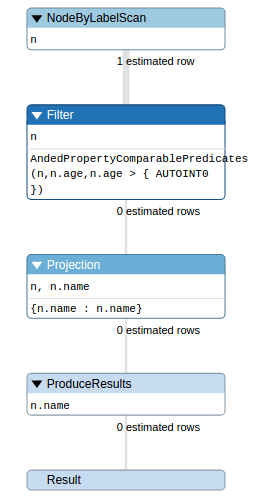
\includegraphics[scale=\screenshotscale]{neo4j-query-plan}
	\caption{Neo4j query plan for \autoref{lst:schema-calculation-example}.}
	\label{fig:neo4-query-plan}
\end{figure}

\begin{figure}
	\centering
	\begin{forest} for tree={align=center}
	[
	{$\production{\var{n.name}}$
		\\ \footnotesize
		$\color{externalschemacolor} \langle \var{n.name} \rangle $
		\\ \footnotesize
		$\color{extravariablescolor} \langle  \rangle $
		\\ \footnotesize
		$\color{internalschemacolor} \langle {}_{0}^{0}
		\var{\var{n.name}}
		\rangle$
	}[
	{$\projection{\var{n.name}}{}
		$
		\\ \footnotesize
		$\color{externalschemacolor} \langle \var{n.name} \rangle $
		\\ \footnotesize
		$\color{extravariablescolor} \langle  \rangle $
		\\ \footnotesize
		$\color{internalschemacolor} \langle {}_{0}^{1}
		\var{\var{n.name}}
		\rangle$
	}[
	{$\selection{
			\var{n.age} > \literal{27}
		}
		$
		\\ \footnotesize
		$\color{externalschemacolor} \langle \var{n}  \rangle $
		\\ \footnotesize
		$\color{extravariablescolor} \langle \var{n.name} \rangle $
		\\ \footnotesize
		$\color{internalschemacolor} \langle {}_{0}^{}
		\var{\var{n} }
		, {}_{1}^{}
		\var{\var{n.name}}
		, {}_{2}^{}
		\var{\var{n.age}}
		\rangle$
	}[
	{$\getvertices{n}{Person}$
		\\ \footnotesize
		$\color{externalschemacolor} \langle \var{n}  \rangle $
		\\ \footnotesize
		$\color{extravariablescolor} \langle \var{n.name}, \var{n.age} \rangle $
		\\ \footnotesize
		$\color{internalschemacolor} \langle {}_{0}^{}
		\var{\var{n} }
		, {}_{1}^{}
		\var{\var{n.name}}
		, {}_{2}^{}
		\var{\var{n.age}}
		\rangle$
	},tier=input,for tree={nullarynodecolor,densely dashed}]
	]
	]
	]
	;
\end{forest}

	\caption{Relational algebra tree with tuples that stand for the \textcolor{externalschemacolor}{external schema}, \textcolor{extravariablescolor}{extra variables} and \textcolor{internalschemacolor}{internal schema}.}
	\label{fig:example-schema-calculation}
\end{figure}

There are three key concepts for defining the schema for each operator in the relational algebra plan:

\begin{itemize}
	\item The \emph{external schema} (typeset in \textcolor{externalschemacolor}{\externalschemacolorname}) is a relational schema that defines the schema visible for users. This schema is what the Neo4j query planner generates (see \autoref{fig:example-schema-calculation}).
	
	\item The \emph{extra variables} (typeset in \textcolor{extravariablescolor}{\extravariablescolorname}) define attributes that are required by an operator's ancestors. For example, the \projectiontext ($\projectionop$) and \selectiontext ($\selectionop$) operators might require additional properties. For \autoref{lst:schema-calculation-example}, the projection requires the $\var{name}$ attribute, while the selection requires the $\var{age}$.
	
	\item The \emph{internal schema} (typeset in \textcolor{internalschemacolor}{\internalschemacolorname}) defines a relational schema that contains the \emph{external schema} plus the extra variables that are required to locally perform computations.
\end{itemize}

\autoref{fig:neo4-query-plan} illustrates these concepts.

We call the process of calculating the external schema, the additional attributes and the internal schema as \emph{schema calculation}.

\section{More examples}

See the Appendices for more examples, starting with the TCK test cases (\autoref{chp:tck}).
